\documentclass[11pt]{article}
\usepackage{graphicx}    % needed for including graphics e.g. EPS, PS
\topmargin -1.5cm        % read Lamport p.163
\oddsidemargin -0.04cm   % read Lamport p.163
\evensidemargin -0.04cm  % same as oddsidemargin but for left-hand pages
\textwidth 16.59cm
\textheight 21.94cm 
%\pagestyle{empty}       % Uncomment if don't want page numbers
\parskip 7.2pt           % sets spacing between paragraphs
%\renewcommand{\baselinestretch}{1.5} % Uncomment for 1.5 spacing between lines
\usepackage{amsmath}
\usepackage{verbatim}
\usepackage{amsfonts}
\usepackage{amsthm}
\usepackage{url}
\parindent 0pt		 % sets leading space for paragraphs
\author{Fermi Ma \and Matt Susskind \and Erik Waingarten}
\title{Playing Ghost in German is PSPACE-Hard}

\newtheorem{theorem}{Theorem}
\newtheorem{lemma}[theorem]{Lemma}
\begin{document}         
\maketitle

\section{Introduction}

	Ghost is a written or spoken word game in which two players take turns adding a letter to the end of a word fragment. The game continues until a valid word is formed and whoever finished the word loses. So each player adds a letter trying to avoid becoming the first to complete a full word. At each turn, the current word fragment must be the prefix of some valid word. If a player believes that his/her opponent has made an invalid move (i.e. the move extends the word fragment so that it is no longer a valid prefix), he/she can use the turn to challenge the other player to name the full word. If the other player can name a valid word, he/she wins the game immediately, and otherwise the challenger wins. In addition, if both players are unaware that a word has just been completed, gameplay continues.

	We consider a more rigid definition of the classic rules. In the version of the game we analyze, we do not allow players to ever make invalid moves or mistakes. We assume that each player knows all the words in the alphabet. This is a reasonable modification to make, as checking the validity of words can easily be done with a dictionary.

	If the entire set of words is considered to be the input to the problem, we can build a game tree which is of polynomial size of the input. A minimax algorithm can find a winning strategy in time polynomial in the size of the input. Thus, the game only becomes interesting from a computational standpoint when the number of words is large. This motivates the need to look at other ways of representing subsets of words. In this paper, we use regular expressions to represent sets of words that are much larger than the input size (the length of the regular expression). A regular expression can work like a dictionary which confirms whether words are in the language.

	Our first result is that given a regular language, it is PSPACE-hard to determine whether a given player has a winning strategy when playing with that language. We use the first result to prove an analogous result for a specific language. In particular, we show that when the game is played on subsets of the German language, it is PSPACE-hard to determine whether a given player has a winning strategy.

\section{PSPACE-hardness of Ghost}
We consider the following instance of the game:

Given any regular expression $R$ and players 1 and 2, does player 1 have a winning strategy in Ghost when played in the language generated by $R$? Player 1 starts.
\begin{theorem} Determining whether player 1 has a winning strategy when Ghost is played over regular languages is PSPACE-hard.
\end{theorem}
\begin{proof} We prove this via reduction from Generalized Geography, a problem known to be PSPACE-hard \cite{theoryofcomp}. Recall that the problem is set up as follows:
Players 1 and 2 take turns moving a token from vertex to vertex in a directed graph G, where player 1 starts the token at a specified start node $s$. A player loses when they are unable to move the token to a vertex that did not have a token previously. Given an instance of the problem, $(G,s)$, can player 1 win the game?

We will use the graph $G$ to build a non-deterministic finite automaton (NFA) that will give a regular expression to play Ghost with. This construction will give an equivalence between games played in Generalized Geography and Ghost, so a winning strategy in one will correspond to a winning strategy in the other and vice versa. To do so, we first label all the edges of $G$ arbitrarily. These labels will represent transitions in the NFA.

We start building the NFA by redrawing the graph $G$, except as a diagram for the NFA. This means that vertices of $G$ are drawn as states of the NFA, and the directed edges turn into transitions between states where transitions are labeled with the same labels given to the corresponding edges in $G$. We then extend construction: for each node $x\in G$, we make another copy of $G$, which we call $G_x$, and make it part of the NFA. For any directed edge $(x,a)$ pointing away from $x$ with label $l$, we make a transition from $x$ to $a'$ in $G_x$ with label $l$, where the prime denotes a corresponding vertex in $G_x$. In addition, we make $x' \in G_x$  the only accept state among the states in $G_x$. If $x\in G$ has no outgoing edges, then corresponding $x$ state in the NFA will have a transition to an accept state $y$ labeled with all possible labels. An example of the contruction is given in Figure~\ref{fig:instance} and Figure~\ref{fig:reduction}. In Figure~\ref{fig:reduction}, the solid transitions correspond to the transitions from $G$ and the dashed transitions correspond to the transitions to the copies of $G$.

From this NFA, we can generate an equivalent regular expression in polynomial time \cite{theoryofcomp}.
\begin{figure}
\centering
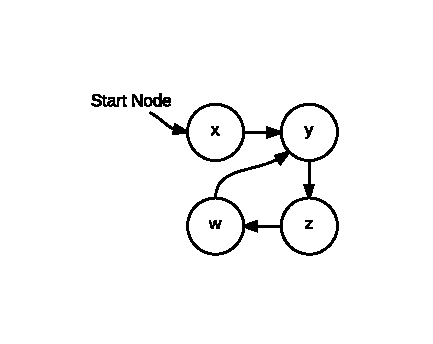
\includegraphics[width=0.3\linewidth]{Ghost1.pdf}
\caption{Instance of Generalized Geography}
\label{fig:instance}
\end{figure}

\begin{figure}
\centering
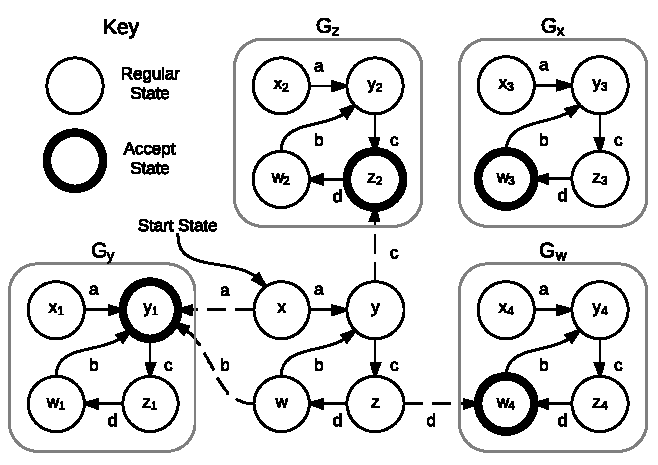
\includegraphics[width=0.6\linewidth]{Ghost2.pdf}
\caption{Corresponding NFA.}
\label{fig:reduction}
\end{figure}

We claim that a winning strategy for Generalized Geography corresponds to a winning strategy for Ghost, played on the language generated by the corresponding NFA. Each move a player makes in Generalized Geography, corresponds to reading a label in the NFA. Once a player reaches a node in Generalized Geography that has no usable outgoing edges (and has thus won), the opposing player in the corresponding Ghost game is forced to move to an accept state in the following move, which spells out a word and loses the game for that player. 

For the other direction of the equivalence, a winning strategy in Ghost (played on the language of the NFA that corresponds to an instance of Generalized Geography) gives a winning strategy in Generalized Geography. The winning strategy in Ghost played on the NFA is to follow valid edges and to avoid ever getting to the accept state of some $G_x$, which corresponds to going back to the same vertex in Generalized Geography.

Thus, the proof follows. 
\end{proof}

It turns out that the idea behind the proof of Theorem 1 can be used to show that Ghost is PSPACE-hard when played on subsets of the German language. We choose to focus on the German language because in German, multiple nouns can always be concatenated together to make new nouns. For example, ``wort", ``band", and ``teil" are all valid German nouns, and thus concatenations such as “wortband” and “wortteilband” are also valid nouns \cite{german}. Therefore, we can describe subsets of the German language with regular expressions.

We consider the following instance of Ghost: The game is played over a given subset of the German language. Does player 1 have a winning strategy if he/she is first to pick a letter?

\begin{theorem}Determining whether player 1 has a winning strategy when Ghost is played over subsets of the German language is PSPACE-hard.
\end{theorem}

\begin{proof} The reduction is very similar in structure to the reduction used in the proof of Theorem 1. However, here we consider Planar Generalized Geography, which is still PSPACE-hard \cite{Sipser}. Given an instance of Planar Generalized Geography, we can four-color the graph in polynomial time \cite{planargraph}. Each edge is then labeled with the color of the vertex it points to. Given this labeling of the graph, we build a corresponding NFA following the procedure in the proof of Theorem 1. The only change we make is that the labels in the graph are mapped to German nouns of odd length that start with different letters. We choose the nouns ``krankenhaus" (hospital), ``wiedervereinigung" (reunification), ``tod" (death), and ``m{\"a}dchen" (girl). Thus, all edges that are colored one color will give transitions labeled with ``tod"��, for example. 

	The German language allows nouns to be concatenated, so the subset of words that are accepted in the NFA are grammatically valid German words. Since the words are all of odd length, when the word finishes, the next player can pick the next word. This corresponds to picking an edge in the NFA, except each transition may take multiple turns. Also, since the starting letter of the words are different, once you start a word, the whole word is specified. This construction builds an NFA that accepts a subset of the words in the German language. 
\end{proof}
\section{Conclusion}

We determined that playing Ghost over regular languages is PSPACE-hard, and we used the same reduction structure to show that Ghost played over subsets of the German language is also PSPACE-hard. The first result is somewhat abstract, as Ghost is generally not played over arbitrary regular languages. However, the second result indicates that there may be other real-world languages that Ghost is hard to play over.

\bibliography{references}
\bibliographystyle{plain}

\end{document}









